\subsection{Login Test Runs}
This subsection contains the test runs for the login screen, using as a reference the login screen test plan available at 13.1.

\subsubsection{Load Quizzes}
This test ensures that a list of all available quizzes can be searched for and found on the login screen, ready to either edit or delete.

\begin{figure}[!htbp]
\centering
\begin{subfigure}{0.5\textwidth}
  \centering
  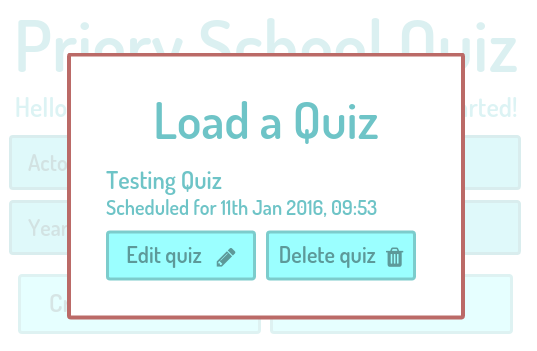
\includegraphics[width=0.95\linewidth]{testing/load_quiz/single_quiz}
  \caption{Single quiz (typical)}
  \label{fig:sub1}
\end{subfigure}%
\begin{subfigure}{0.5\textwidth}
  \centering
  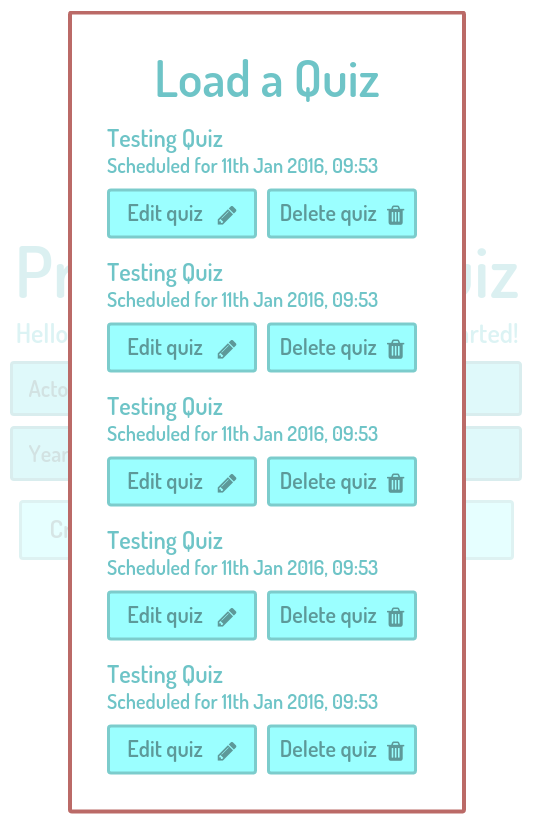
\includegraphics[width=0.95\linewidth]{testing/load_quiz/multiple_quizzes}
  \caption{Five quizzes (extreme)}
  \label{fig:sub2}
\end{subfigure}
\begin{subfigure}{0.5\textwidth}
  \centering
  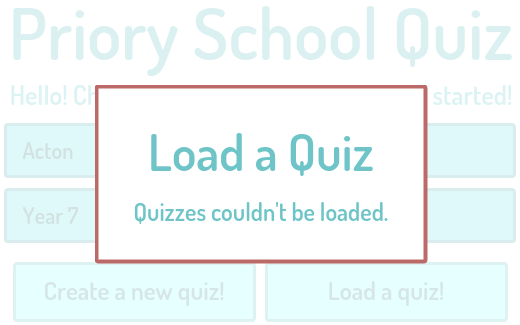
\includegraphics[width=0.95\linewidth]{testing/load_quiz/offline}
  \caption{No connection (erroneous)}
  \label{fig:sub2}
\end{subfigure}
\begin{subfigure}{0.5\textwidth}
  \centering
  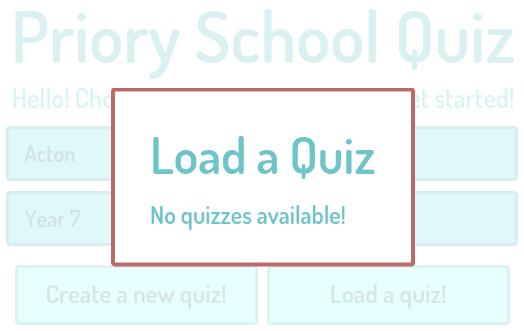
\includegraphics[width=0.95\linewidth]{testing/load_quiz/no_quizzes}
  \caption{No quizzes (null)}
  \label{fig:sub2}
\end{subfigure}
\caption{The load quiz dialog.}
\label{fig:test}
\end{figure}
As can be seen, all the tests have worked successfully: when there is only a single quiz in the database, only a single quiz is shown; when there are five, all of these are listed; when there is no connection, and the system is unable to perform an API call, the correct error message is shown; and when there are simply no quizzes available, this too is properly relayed to the user. \textit{Success.}


\subsubsection{Delete Quizzes}
This test ensures that the user is able to delete a quiz from the database, using the button in the load quiz dialog.

\begin{figure}[!htbp]
\centering
\begin{subfigure}{0.5\textwidth}
  \centering
  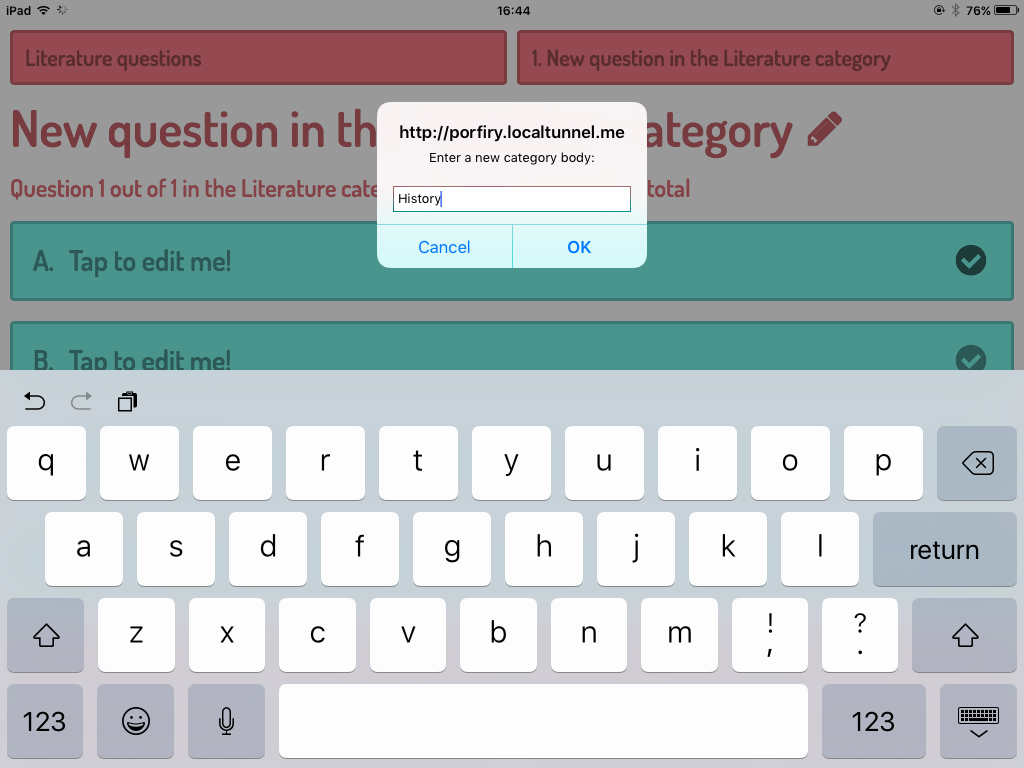
\includegraphics[width=0.95\linewidth]{testing/delete_quiz/during}
  \caption{During}
  \label{fig:sub1}
\end{subfigure}%
\begin{subfigure}{0.5\textwidth}
  \centering
  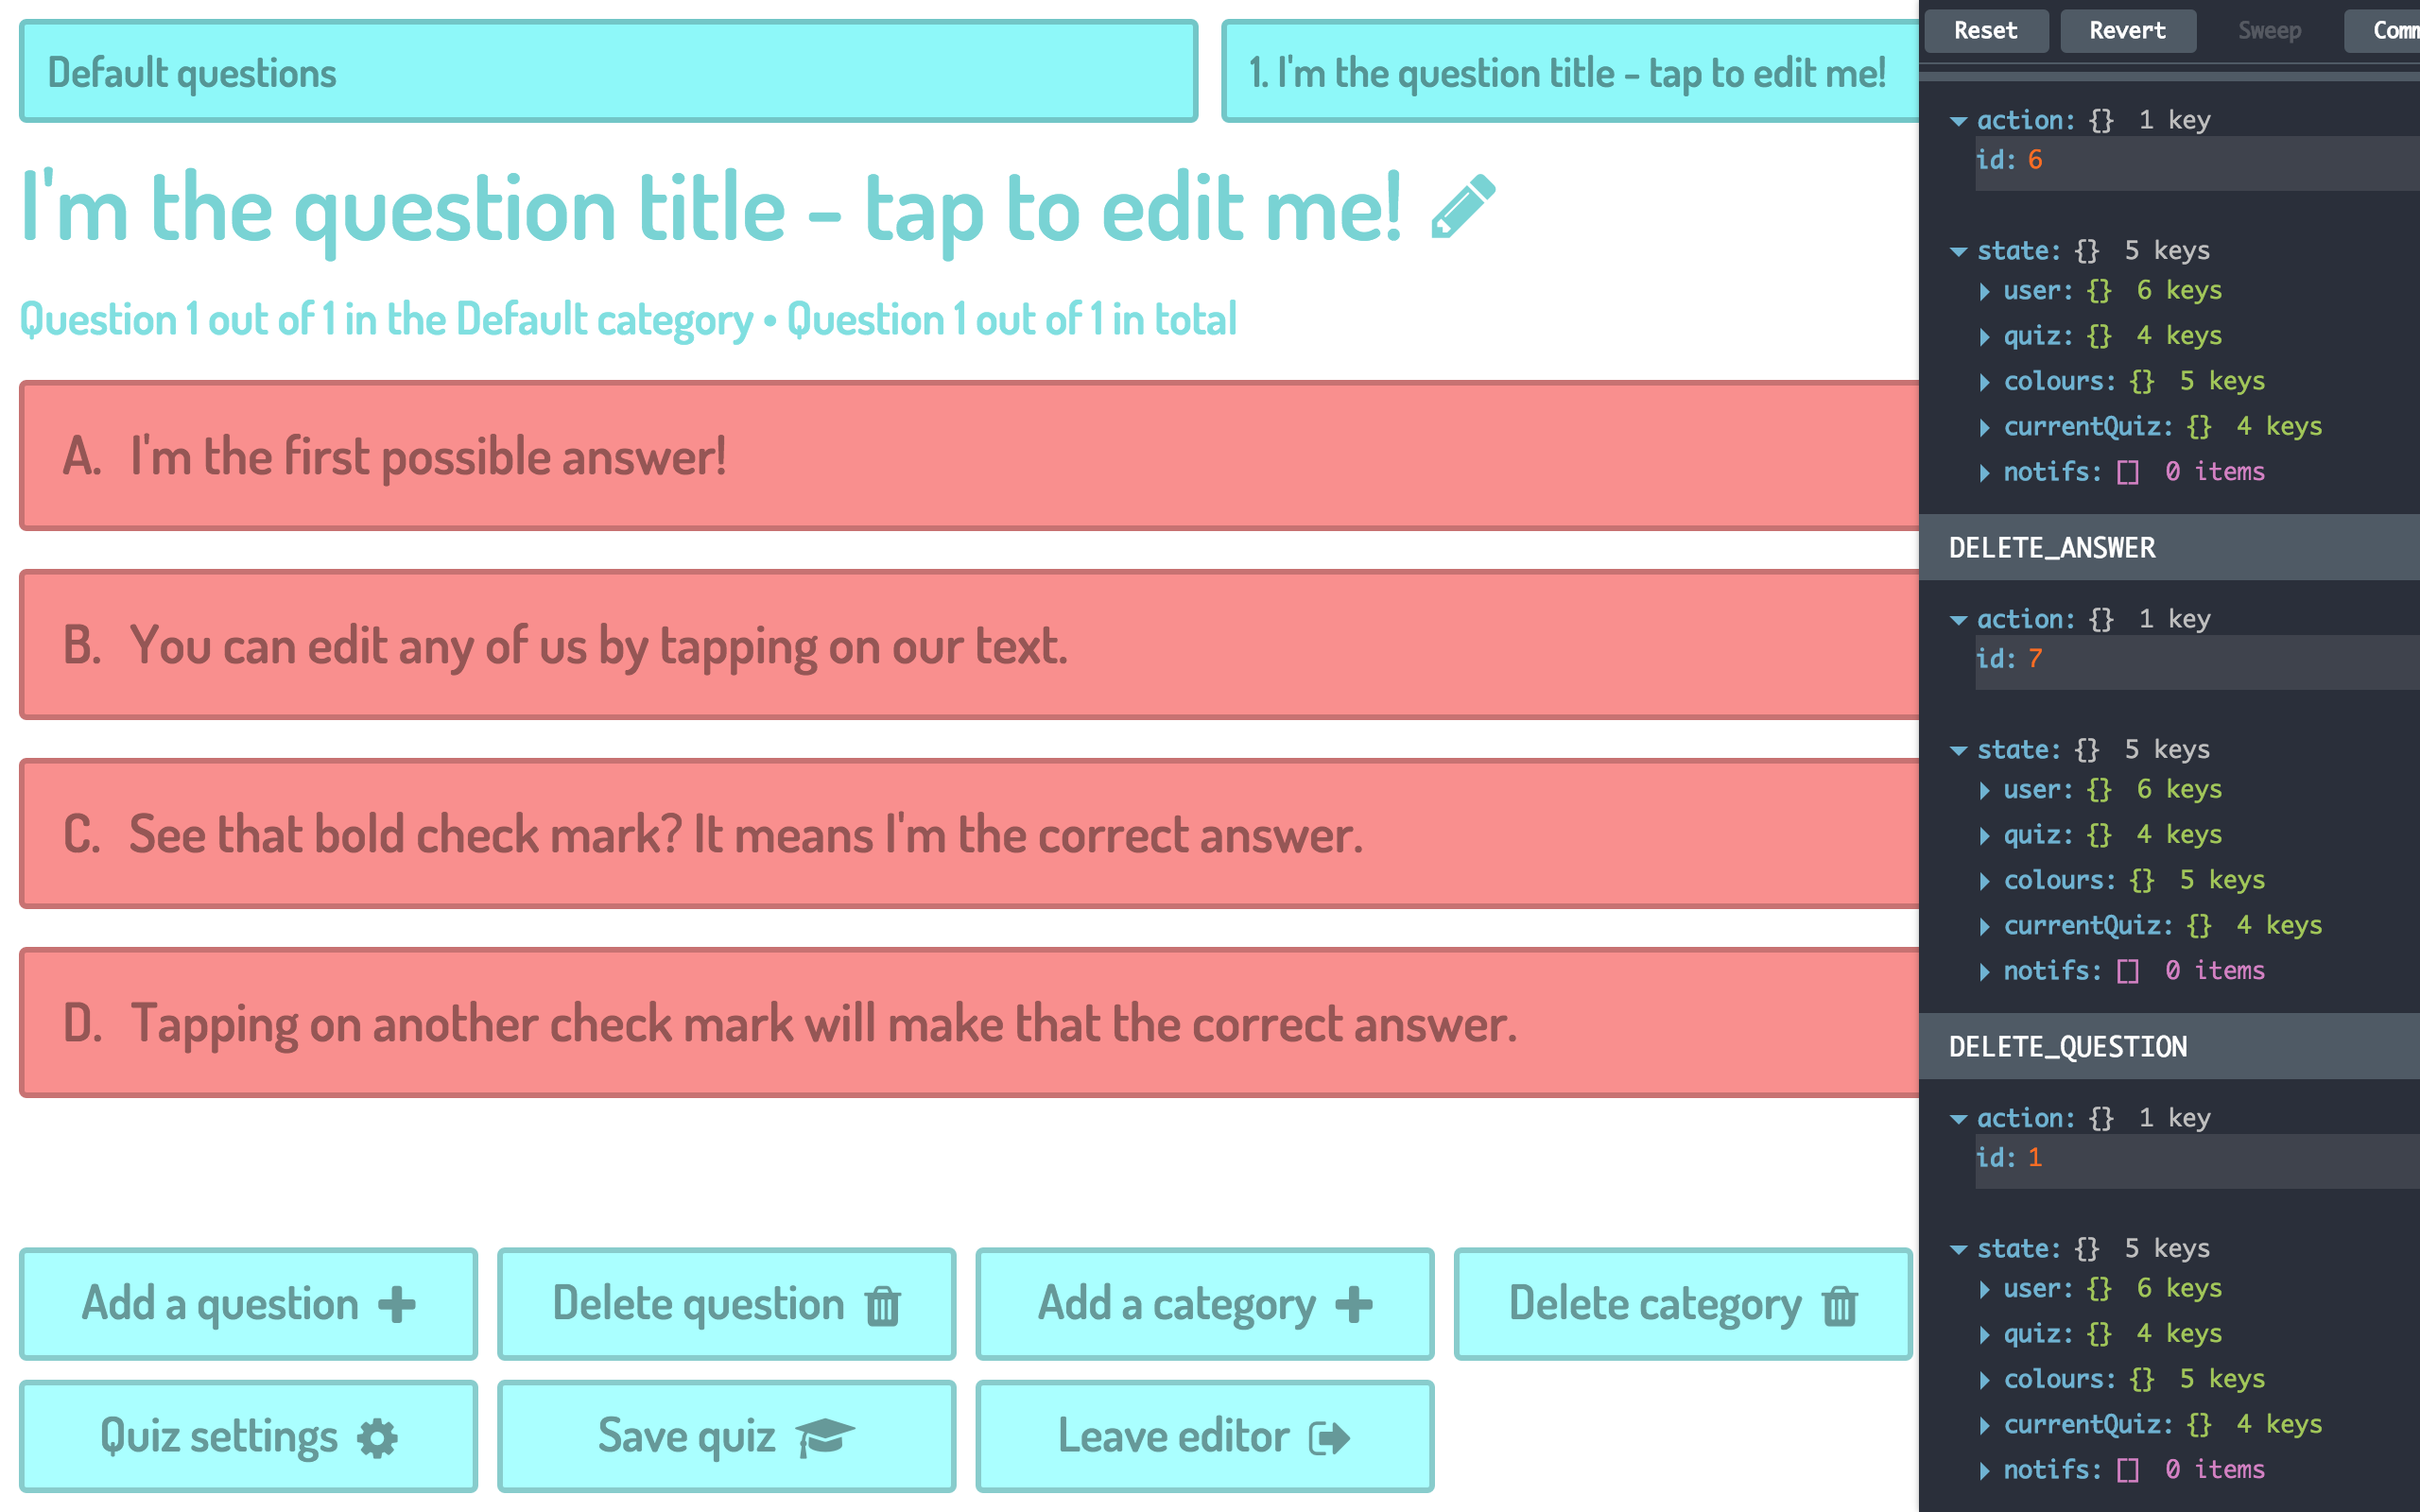
\includegraphics[width=0.95\linewidth]{testing/delete_quiz/after}
  \caption{Five quizzes (extreme)}
  \label{fig:sub2}
\end{subfigure}
\begin{subfigure}{0.5\textwidth}
  \centering
  \includegraphics[width=0.95\linewidth]{testing/delete_quiz/database}
  \caption{Database view}
  \label{fig:sub2}
\end{subfigure}
\caption{The load quiz dialog.}
\label{fig:test}
\end{figure}
